\chapter{Elaborazione di immagini lunari} \label{chap:techniques}

Questo capitolo si propone di approfondire le tecniche di elaborazione delle immagini lunari, illustrando le nozioni teoriche alla base degli algoritmi implementati nel progetto. Ogni tecnica verrà descritta in dettaglio, partendo da calibrazione e allineamento, passando per pre-processing e stacking, per concludere con il post-processing. Quando necessario, verranno forniti pseudocodice e descrizioni dei processi matematici applicati alle immagini; l'implementazione sarà invece discussa nel capitolo \ref{chap:implementation}.

\section{Calibrazione di immagini} \label{sec:calibration}

La \textbf{calibrazione} delle immagini è un passaggio fondamentale nell'astrofotografia, necessario per rimuovere rumore e artefatti introdotti dalla strumentazione. In particolare, nel contesto delle immagini lunari, la calibrazione è utile per rimuovere il rumore termico e i difetti del sensore, oltre a uniformare l'illuminazione dell'immagine. Questo processo è composto da tre fasi principali: la cattura di \textit{bias frames}, \textit{dark frames} e \textit{flat frames}. Tali scatti devono essere acquisiti con la fotocamera nello stesso stato in cui sono state scattate le immagini lunari, in particolare nelle stesse condizioni termiche. Infatti, quando viene eseguita una sessione di molti scatti, o con lunghe esposizioni, la macchinetta tende a scaldarsi causando effetti non sempre trascurabili, e sono proprio quelli che vogliamo mitigare mediante la fase di calibrazione. In questa fase gli scatti della luna vengono denominati \textit{light frames}.

\subsection{Bias Frames} \label{subsec:bias}

I \textbf{bias frames} son scatti acquisiti con il tempo di esposizione più breve possibile (il minimo supportato dalla macchina fotografica, idealmente zero), ISO uguale a quello dei light frames e con l'otturatore della fotocamera chiuso. Questi frame catturano il \textbf{rumore di bias}, un segnale di offset introdotto dall'elettronica del sensore in assenza di luce. Il rumore di bias è presente in tutte le immagini acquisite con una macchina fotografica, e varia leggermente da pixel a pixel \cite{calibration}.

Per correggere questo rumore si calcola il cosiddetto \textbf{master bias} combinando i diversi bias frames, generalmente calcolandone la media. Il master bias viene poi sottratto da tutte le immagini acquisite, inclusi gli altri frame di calibrazione.

\begin{algorithm}[H]
    \caption{Calcolo del master bias} \label{alg:bias}
    \textbf{Input:} \Comment{Lista di bias frames} \\
    \textbf{Ouput:} \Comment{Master bias calcolato}
    \begin{algorithmic}[1]
        \Function{calculate\_master\_bias}{$B_f$}
            \State $N \gets$ \text{numero di bias frames}
            \State $M_b \gets 0$
            \For{$i \gets 1$ to $N$}
                \State $M_b \gets M_b + \dfrac{B_f[i]}N$ \Comment{Media dei bias frames}
            \EndFor
            \State \textbf{return} $M_b$
        \EndFunction
    \end{algorithmic}
\end{algorithm}

\textbf{Applicazione:} Per applicare il master bias a un'immagine, si sottrae semplicemente il master bias dall'immagine originale. In formula, data un'immagine \textit{original} e il master bias \textit{master\_bias}, l'immagine calibrata \textit{final\_image} sarà data da:

$$
    final\_image = original - master\_bias
$$

\subsection{Dark Frames} \label{subsec:dark}

I \textbf{dark frames}, acquisiti con stessi ISO e tempi di cattura dei light frames, ma con l'otturatore chiuso, catturano il \textbf{rumore termico} causato dall'agitazione termica degli elettroni nel sensore. Questo rumore aumenta con il tempo di esposizione e con la temperatura del sensore e può variare significativamente tra scatti differenti.

Per correggere il rumore termico, si calcola il \textbf{master dark} combinando i diversi dark frames, generalmente calcolandone la media. Il master dark viene poi sottratto ai light frames e ai flat fames. È importante sottrarre il master bias dai dark frames prima di calcolare il master dark, per evitare di sommare due volte il rumore di bias.

\begin{algorithm}[H]
    \caption{Calcolo del Master Dark}
    \textbf{Input:} $D_f$ \Comment{Lista di dark frames} \\
    \textbf{Ouput:} $M_d$ \Comment{Master dark calcolato}
    \begin{algorithmic}[1]

        \Function{calculate\_master\_dark}{$D_f$}
            \State $N \gets$ \text{numero di dark frames}
            \State $M_d \gets 0$
            \For{$i \gets 1$ to $N$}     
                \State $ D_c \gets D_f[i] - M_b$ \Comment rimozione del bias
                \State $M_d \gets M_d + \dfrac {D_c} N$ \Comment media dei dark frames
            \EndFor
            \State \textbf{return} $M_d$
        \EndFunction
    \end{algorithmic}
\end{algorithm}

\textbf{Applicazione:} Per applicare il master dark a un'immagine, si sottrae semplicemente il master dark dall'immagine originale. In formula, data un'immagine \textit{original} e il master dark \textit{master\_dark}, l'immagine calibrata \textit{final\_image} sarà data da:

$$
    final\_image = original - master\_dark
$$

\subsection{Flat Frames} \label{subsec:flat}

I \textbf{flat frames} sono scatti acquisiti fotografando una sorgente di luce uniforme, come un cielo crepuscolare o un pannello luminoso. Vengono acquisiti con lo stesso tempo di esposizione e ISO dei light frames, ma con l'otturatore aperto. Questi frame catturano le variazioni nella risposta dei pixel del sensore e il \textbf{rumoe di vignettatura} introdotto dal sistema ottico, ovvero la diminuzione dell'illuminazione verso i bordi dell'immagine.

Per correggere queste imperfezioni si calcula un \textbf{master flat} combinando i diversi flat frames, solitamente attraverso la media. Prima di calcolare il master flat, è necessario sottrarre sia il master bias che il master dark dai flat frames. Una volta calcolato il master flat, questo viene normalizzato dividendolo per il valore medio dei suoi pixel. Il master flat viene poi utilizzato per normalizzare le immagini scientifiche, dividendo ogni pixel dell'immagine per il corrispondente valore nel master flat.

\begin{algorithm}[H]
    \caption{Calcolo del Master Flat}
    \textbf{Input:} $F_f$ \Comment{Lista di flat frames} \\
    \textbf{Ouput:} $M_f$ \Comment{Master flat calcolato}
    \begin{algorithmic}[1]
        \Function{calculate\_master\_flat}{$F_f$}
            \State $N \gets$ \text{numero di flat frames}
            \State $M_f \gets 0$
            \For{$i \gets 1$ to $N$}
                \State $F_c \gets F_f[i] - M_b - M_d$ \Comment{rimozione di bias e dark}
                \State $M_f \gets M_f + \dfrac {F_c} N$ \Comment{media dei flat frames}
            \EndFor
            \State $M_f \gets \dfrac {M_f} {\text{mean}(M_f)}$ \Comment{normalizzazione}
            \State \textbf{return} $M_f$
        \EndFunction
    \end{algorithmic}
\end{algorithm}

\textbf{Applicazione:} Per applicare il master flat a un'immagine, si divide semplicemente l'immagine originale:

$$
    final\_image = \dfrac {original} {M_f}
$$

Nel contesto di questo progetto, i flat frames non sono stati acquisiti per due principali motivi. In primo luogo, la loro acquisizione risulta complessa e richiede condizioni specifiche che non sono state facilmente riproducibili durante le sessioni fotografiche. In secondo luogo, l'effetto della vignettatura non ha rappresentato un problema significativo nelle immagini ottenute, poiché la Luna era posizionata verso il centro degli scatti e occupava meno di un terzo dell'altezza dell'immagine. Nonostante ciò, il processo di calibrazione è stato comunque implementato per consentire l'utilizzo di flat frames, garantendo flessibilità e scalabilità del metodo di elaborazione adottato.

\subsection{Processo completo di calibrazione} \label{subsec:calibration_process}

Il processo completo di calibrazione applica in sequenza le correzioni con i master frames; si sottrae il master bias, si sottrae il master dark e si divide per il master flat:

\begin{algorithm}[H]
    \caption{Calibrazione di un'immagine}
    \textbf{Input:} $Img$ \Comment{Immagine da calibrare} \\
    \phantom{Input: } $M_b$ \Comment{Master bias} \\
    \phantom{Input: } $M_d$ \Comment{Master dark} \\
    \phantom{Input: } $M_f$ \Comment{Master flat} \\
    \textbf{Ouput:} $Out$ \Comment{Immagine calibrata}
    \begin{algorithmic}[1]
        \Function{calibrate\_image}{$Img, M_b, M_d, M_f$}
            \State $Out \gets \dfrac {Img - M_b - M_d} {M_f}$
            \State \textbf{return} $Out$
        \EndFunction
    \end{algorithmic}
\end{algorithm}

\textbf{Applicazione:} Per calibrare un'immagine, si applica la funzione \textit{calibrate\_image} con i master frames calcolati. In formula, data un'immagine \textit{original} e i master frames $M_b$, $M_d$ e $M_f$, l'immagine calibrata \textit{final\_image} sarà data da:

$$
    final\_image = \dfrac {original - M_b - M_d} {M_f}
$$

Questo processo (illustrato in figura \ref{fig:calibration})  permette di ottenere immagini corrette da rumori elettronici, termici e da imperfezioni ottiche.

\begin{figure} [H]
    \centering
    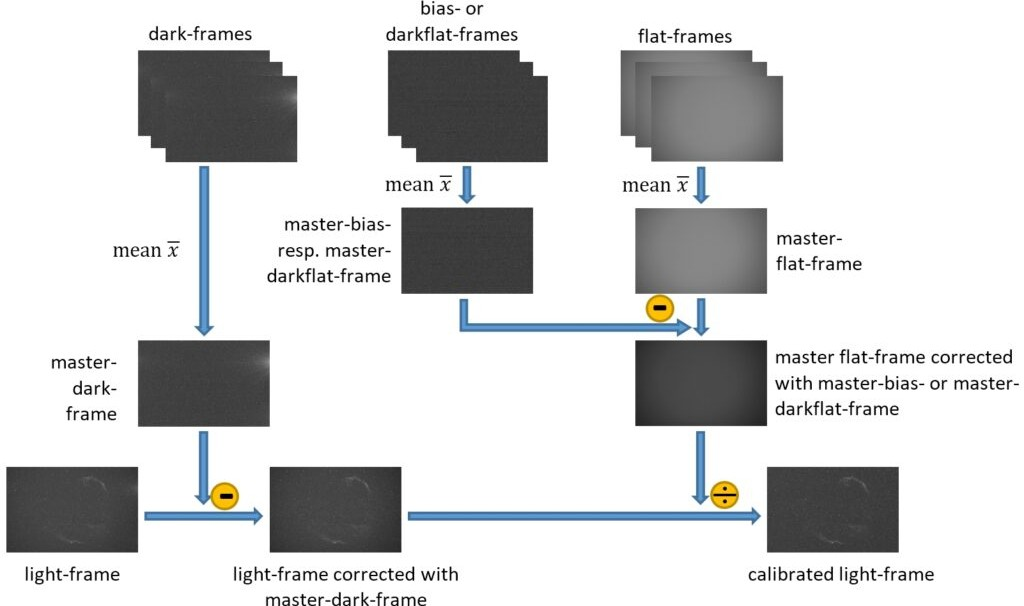
\includegraphics[scale = 0.33]{../assets/calibration_procedure.jpg}
    \captionsetup{justification=centering}
    \caption{Illustrazione schematica dell'uso di immagini di calibrazione \cite{calibration_img}} \label{fig:calibration}
\end{figure}

\section{Allineamento delle immagini} \label{sec:alignment}

\subsection{Feature Detection e Matching ORB, SIFT e SURF} \label{subsec:feature_detectoion}

\subsection{Trasformazioni omografiche} \label{subsec:homography}

\section{Pre-processing delle immagini} \label{sec:preprocessing}

\subsection{Denoising tramite reti neurali: DnCnn} \label{subsec:denoising}

\subsection{Unsharp Masking e personalizzazione} \label{subsec:unsharp_mask}

\section{Stacking delle immagini} \label{sec:stacking}

\subsection{Principi e vantaggi dello stacking} \label{subsec:stacking_intro}

\subsection{Algoritmi di stacking} \label{subsec:atacking_algo}

\section{Post-Processing delle immagini} \label{sec:postprocess}

\subsection{Miglioramento di nitidezza e contrasto} \label{subsec:contrast}

\cleardoublepage